\subsection{Parameter Identification}
\begin{figure}[t]
    \hfill
    \begin{minipage}{\columnwidth}
        \centering
        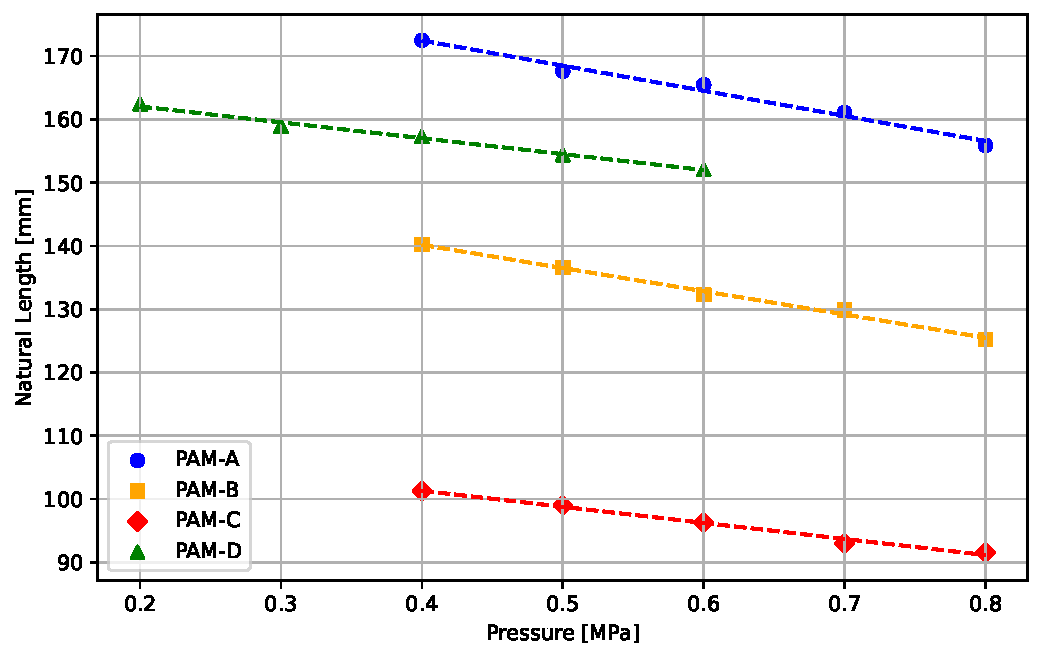
\includegraphics[width=\columnwidth]{fig/length_pressure.pdf} 
        \caption{Linearity of Natural Length to Pressure}
        \label{fig:length_pressure}
        \vspace{1em} 
        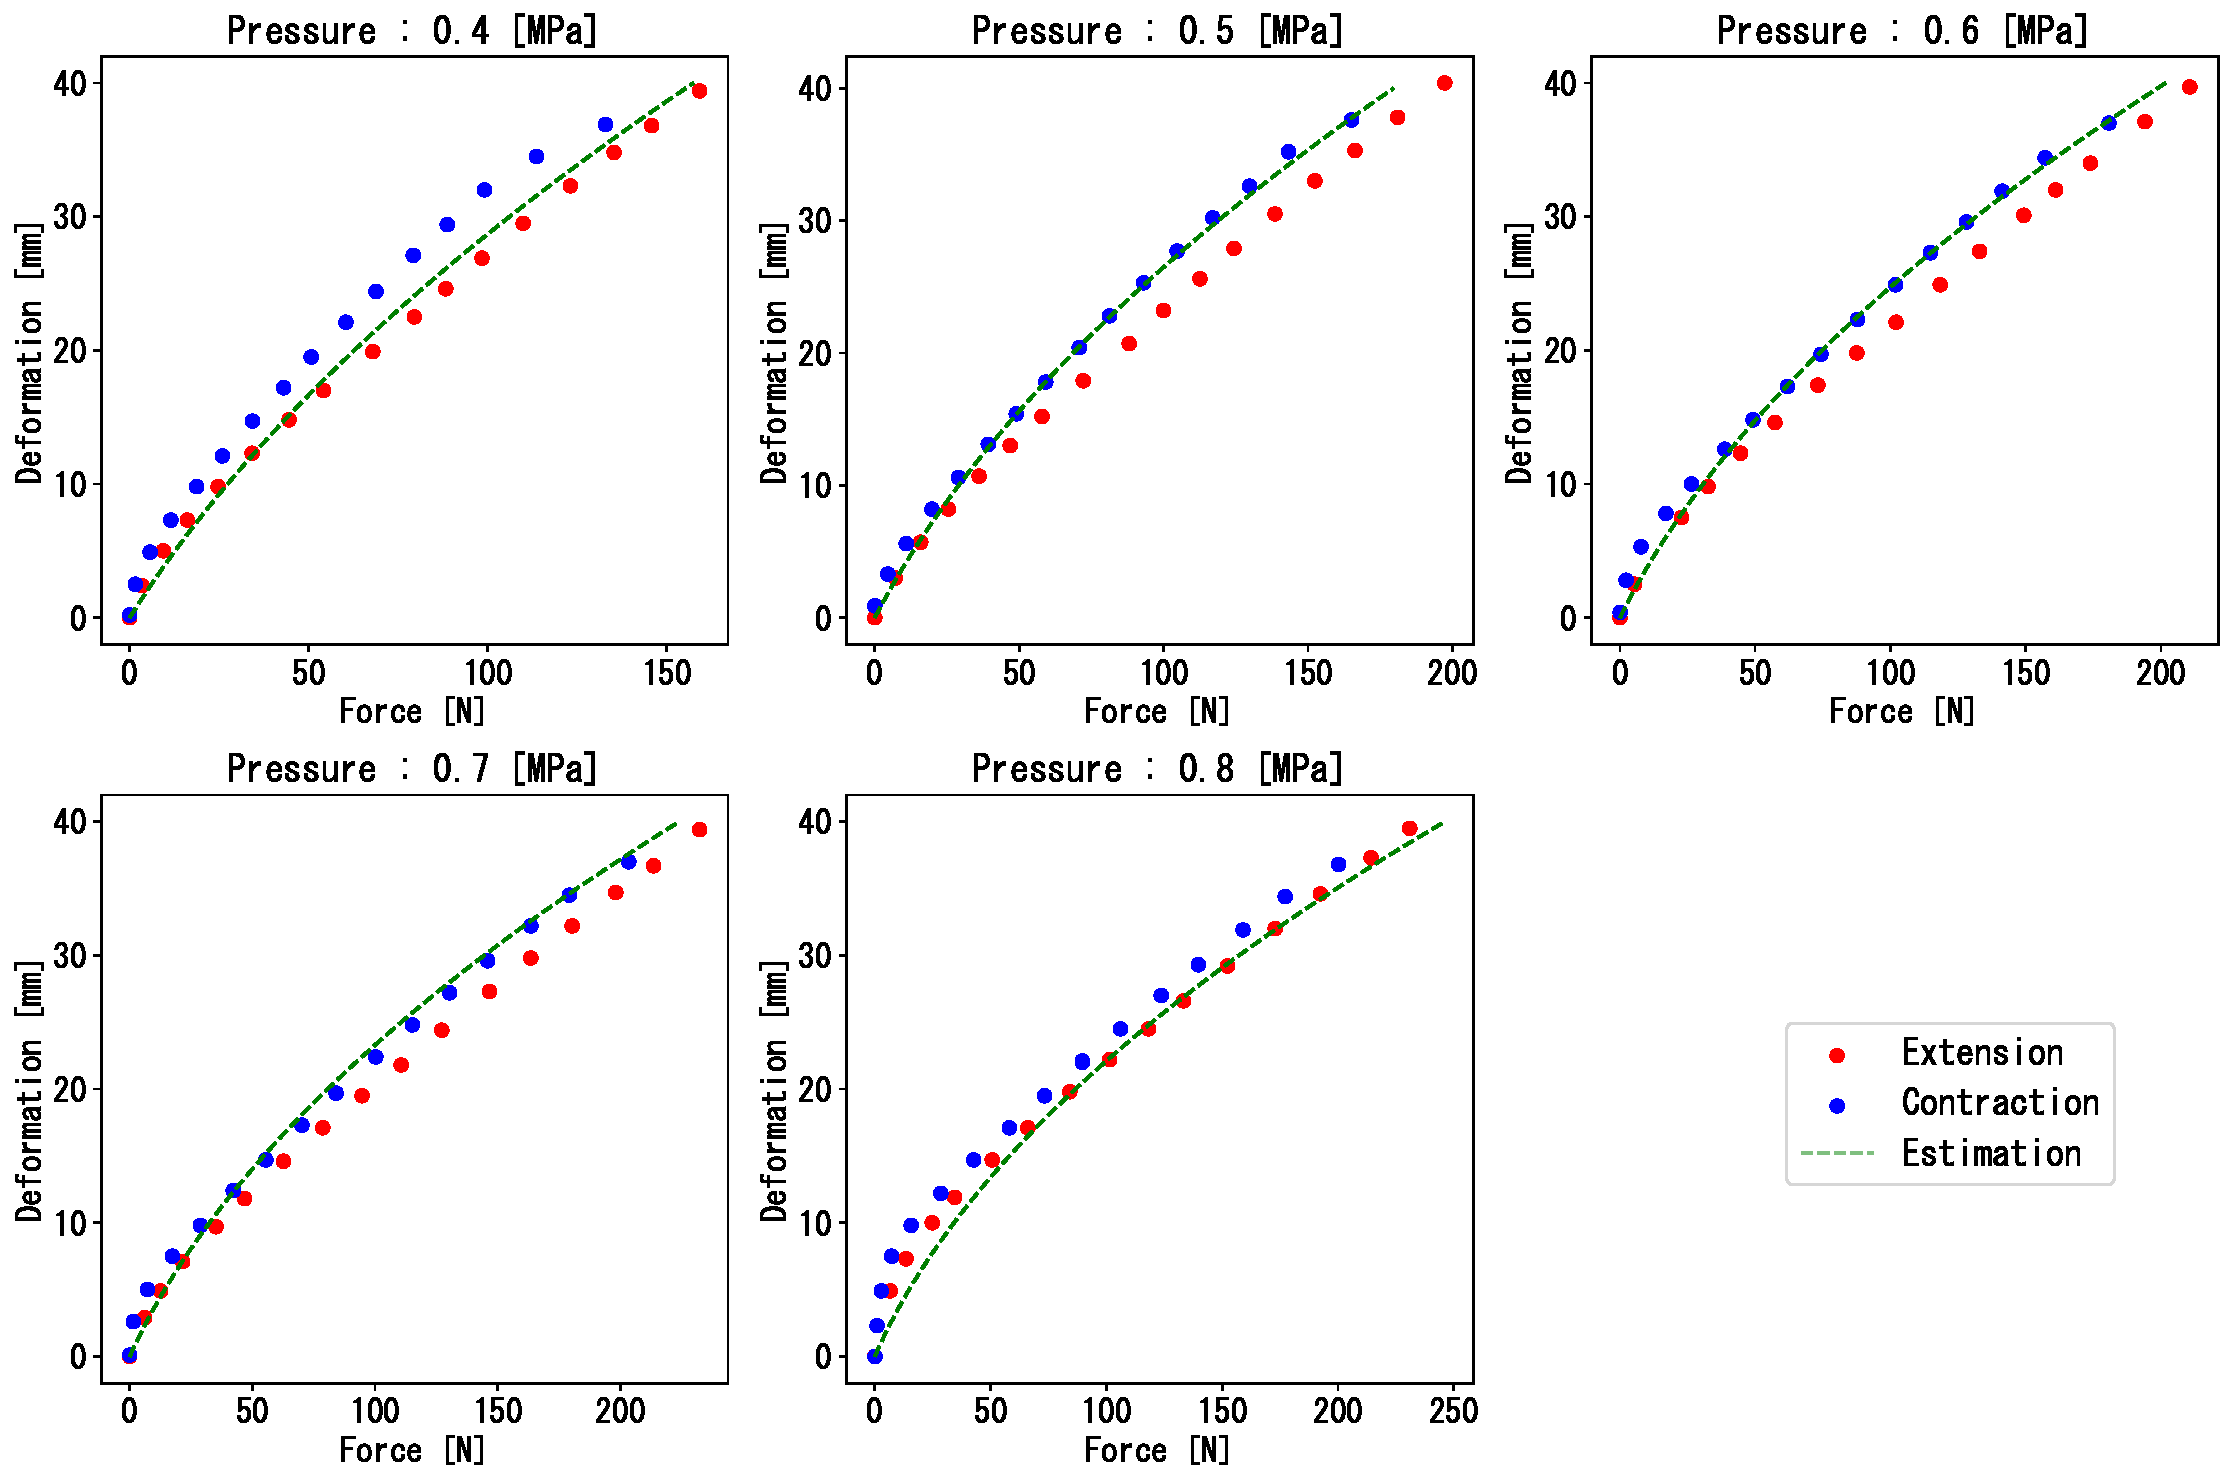
\includegraphics[width=\columnwidth]{fig/20231124_5_4s_2d_ieeesensors1.pdf}
        \caption{Nonlinearity of Deformation under Different Pressure (PAM-B)}
        \label{fig:pam_b_static1}
    \end{minipage}
\end{figure}
\begin{table}[t]
    \centering
    \caption{Parameters for Stretch Reflex} 
    \begin{tabular}{c|cc}
        \hline
        Method &$V_{thr} [\si{mm/s}]$&$ k [\si{GPa\cdot s}]$\\
        \hline \hline
        Model & 70 & 1/800\\
        Fiber Sensor & 25 & 1/300\\
        \hline
    \end{tabular}
\label{tab:reflex_para}
\end{table}
\begin{figure*}[h]
    \begin{center}
        \begin{minipage}[t]{\columnwidth} 
            \centering
            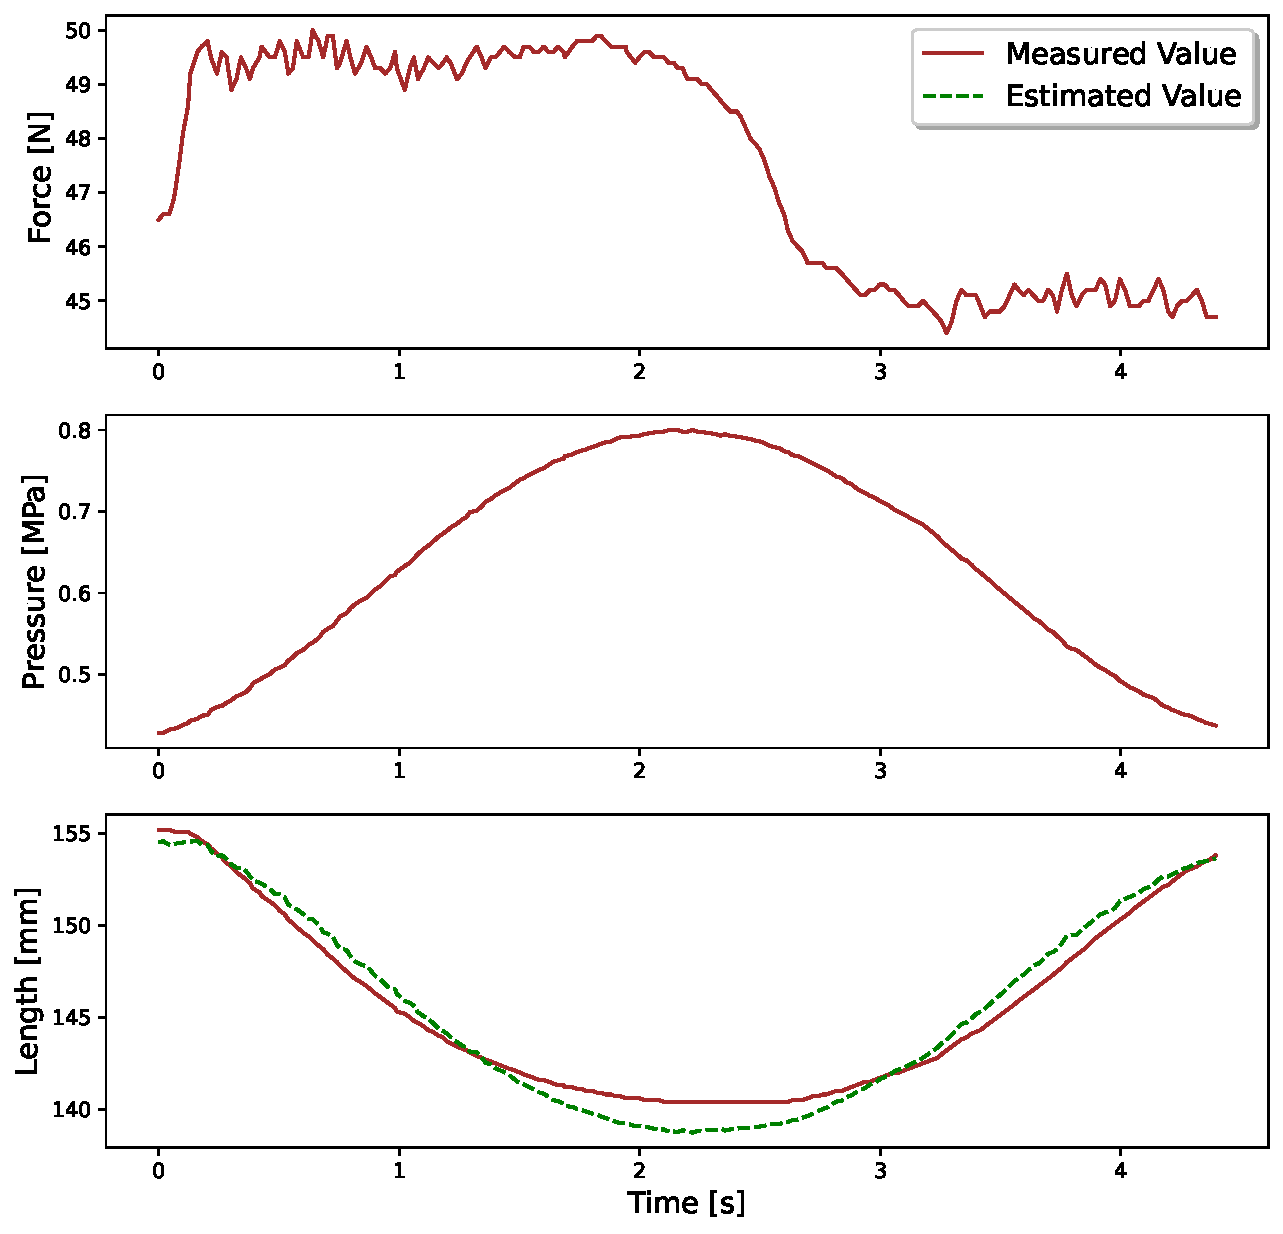
\includegraphics[keepaspectratio, width=\columnwidth]{fig/20231207_1_4s_by_5_2d_ieeesensors2.pdf}
            \caption{Dynamic Length Estimation (PAM-B, Rubber)}
            \label{fig:pam_b_dynamic}
        \end{minipage}
        \hfill
        \begin{minipage}[t]{\columnwidth} 
            \centering
            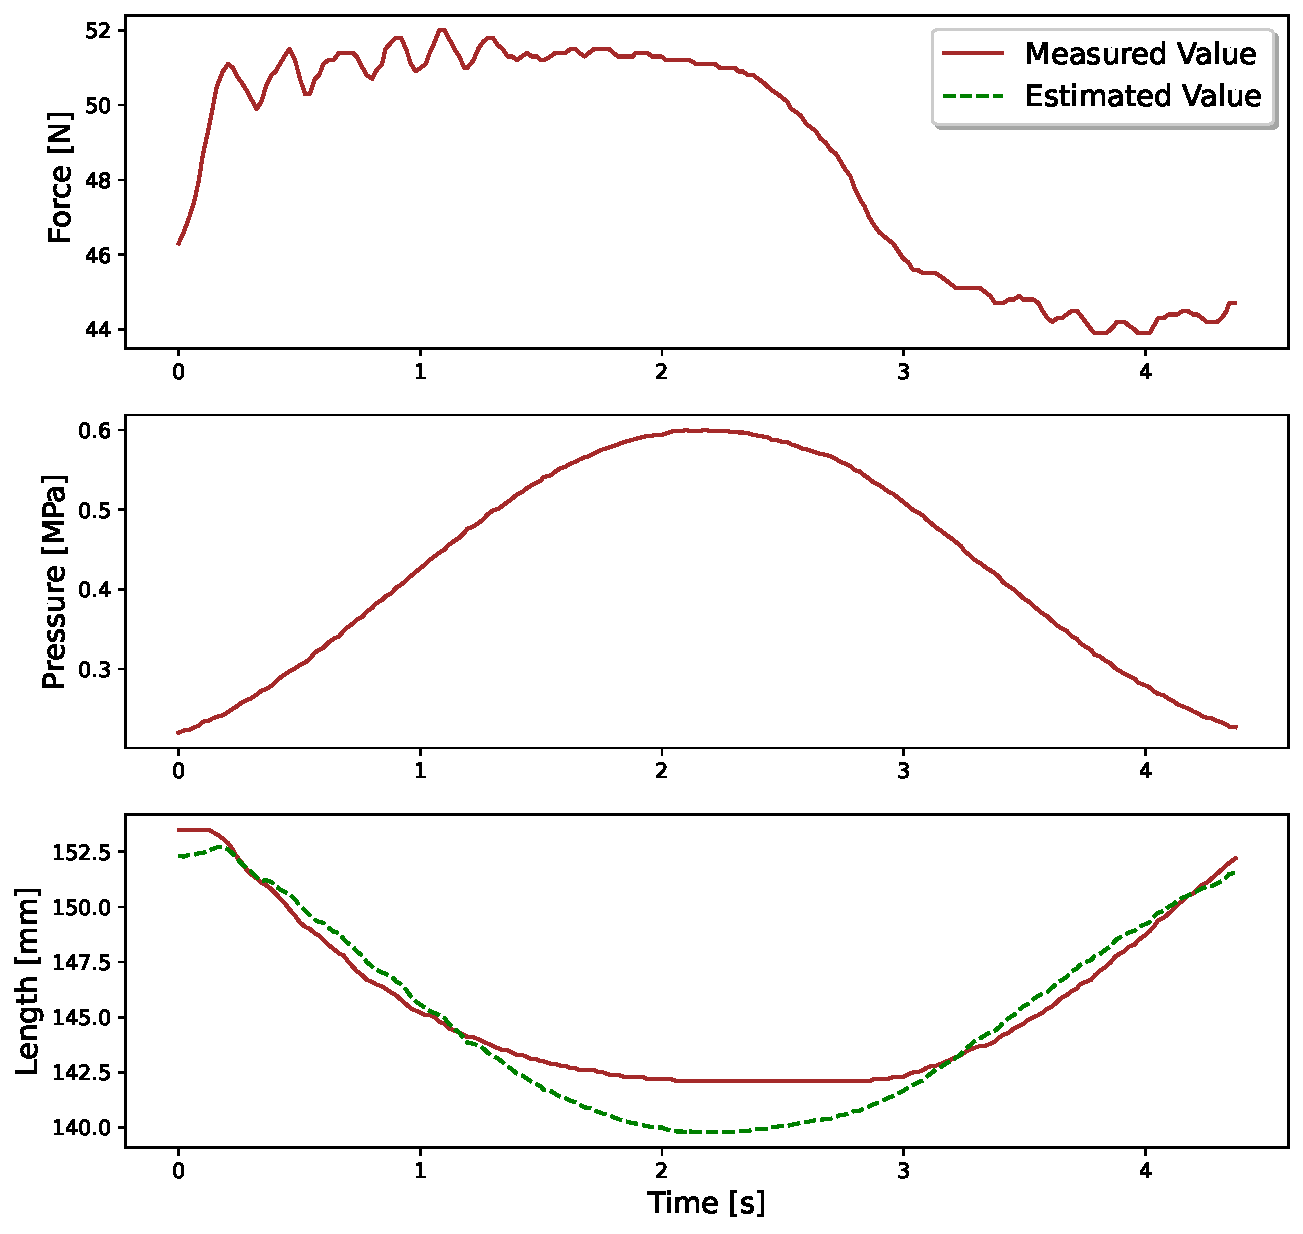
\includegraphics[keepaspectratio, width=\columnwidth]{fig/20231220_2_s_by_2_2d_ieeesensors2.pdf}
            \caption{Dynamic Length Estimation (PAM-D, Silicon)}
            \label{fig:pam_d_dynamic}
        \end{minipage}
    \end{center}
 \end{figure*} 
Fig. \ref{fig:length_pressure} displays the relationship between pressure $p$ and natural length $l_n$ of the PAMs. As assumed, there is a tendency for $l_n$ to decrease linearly with $p$ within the tested pressure range. The dashed lines in Fig. \ref{fig:length_pressure} represent the fitted lines using the least squares method, as expressed by Eq. (\ref{eq:L_n}).
Fig. \ref{fig:pam_b_static1} shows the result of the static tensile test for PAM-B. The red and blue points represent the measurements during expansion and contraction respectively, and the green dashed lines represent the solutions $d$ to Eq. (\ref{eq:model}), which is given by substituting the predetermined parameters $a_i$ and the measured $f$ and $p$.
Generally, PAMs exhibit hysteresis caused by friction, so the data differ between expansion and contraction processes. Due to the space constraint, the result of the static tensile test is only presented for PAM-B, but similar results were obtained for the other PAMs.

\subsection{Dynamic Length Estimation} 
Fig. \ref{fig:pam_b_dynamic} and Fig. \ref{fig:pam_d_dynamic} show the dynamic length estimations for PAM-B and PAM-D, respectively.
By means of the three model equations Eq. (\ref{eq:model}), Eq. (\ref{eq:model_2d(1)}) and Eq. (\ref{eq:model_3d}), with respect to the measurements by the linear encoder, the length estimations were achieved with the maximum errors and the root mean squared errors (RMSEs) as shown in Table \ref{tab:errors}.
   
\subsection{Reaching Task}
Table \ref{tab:parameters} shows the parameters for the length estimations of the agonist and antagonist muscles. The considerable difference in the voltage-force slope $q$ between the two PAMs is attributable to the varying sensitivities of the handmade strain gauges. Fig.\ref{fig:reaching_error} displays the length estimation errors of the model and the fiber sensor in reaching task. Since the fiber sensor could only measure the rate of length change and not the absolute length, the estimations of absolute length by the fiber sensor were calibrated to the measurements of the linear encoder at the start of the reaching task. Therefore, it cannot be said that Fig.\ref{fig:reaching_error} is exactly comparing the estimates from the model and the fiber sensor, but it serves as a reference for examining the accuracy of the model against the conventional sensor. The reaching task was performed five times for both the agonist and antagonist muscles. 
According to the model equation Eq. (\ref{eq:model}), compared with the measurements from the linear encoder, the length estimations showed the maximum errors and the root mean squared errors (RMSEs) as illustrated in Table \ref{tab:errors2}.
\begin{table}[t]
    \centering
    \caption{Error Percentages of Dynamic Length Estimations under Different Model Equations}
    \label{tab:errors}
    \resizebox{\columnwidth}{!}{%
    \begin{tabular}{c|cccccccc}
    \hline
    \multirow{2}{*}{Model} & \multicolumn{2}{c}{PAM-A} & \multicolumn{2}{c}{PAM-B} & \multicolumn{2}{c}{PAM-C} & \multicolumn{2}{c}{PAM-D} \\ 
    \cline{2-9}
                           & Max & RMSE & Max & RMSE & Max & RMSE & Max & RMSE \\ 
    \hline
    \hline
    Eq. (3) & 1.72 & 0.861 & 1.19 & 0.653 & 1.18 & 0.683 & 1.65 & 0.846 \\ 
    Eq. (4) & 1.12 & 0.633 & 0.773 & 0.353 & 1.01 & 0.548 & 0.755 & 0.435 \\ 
    Eq. (5) & 1.22 & 0.516 & 1.41 & 0.484 & 0.951 & 0.500 & 1.99 & 0.606 \\ 
    \hline
    \end{tabular}%
    }
\end{table}
\begin{table}[t]
    \centering
    \caption{Parameters for Length Estimations in Reaching Task} 
    \resizebox{\columnwidth}{!}{%
    \begin{tabular}{c|ccccccc}
        \hline
        PAM & $m$ & $h$ & $a_3$ & $a_2$ & $a_1$ & $a_0$ & $q$ \\
        \hline \hline
        Agonist & -60.1 & 170.1 & -0.201 & 7.00 & 0.256 & 0.911 & $2.25 \times 10^{-3}$\\
        Antagonist & -70.3 & 178.5 & 0.871 & 1.24 & -0.129 & 22.4 & $4.33 \times 10^{-3}$ \\
        \hline
    \end{tabular}
    } 
    \label{tab:parameters}
\end{table}
\begin{table}[H]
    \centering
    \caption{Error Percentages of Length Estimations in Reaching Task}
    \label{tab:errors2}
    \resizebox{\columnwidth}{!}{%
    \begin{tabular}{c|cccc}
    \hline
    \multirow{2}{*}{Method} & \multicolumn{2}{c}{Agonist} & \multicolumn{2}{c}{Antagonist} \\ 
    \cline{2-5}
                                 & Max  & RMSE  & Max   & RMSE  \\ 
    \hline
    \hline
    Model Eq. (\ref{eq:model}) & 8.82 & 5.24 & 5.86 & 5.02 \\ 
    Fiber Sensor & 2.51 & 0.888 & 2.53 & 1.78 \\ 
    \hline
    \end{tabular}%
    }
\end{table}
\begin{figure*}[t]
    \centering
    \begin{minipage}[H]{\textwidth} 
        \begin{minipage}[H]{0.48\textwidth} 
            \centering
            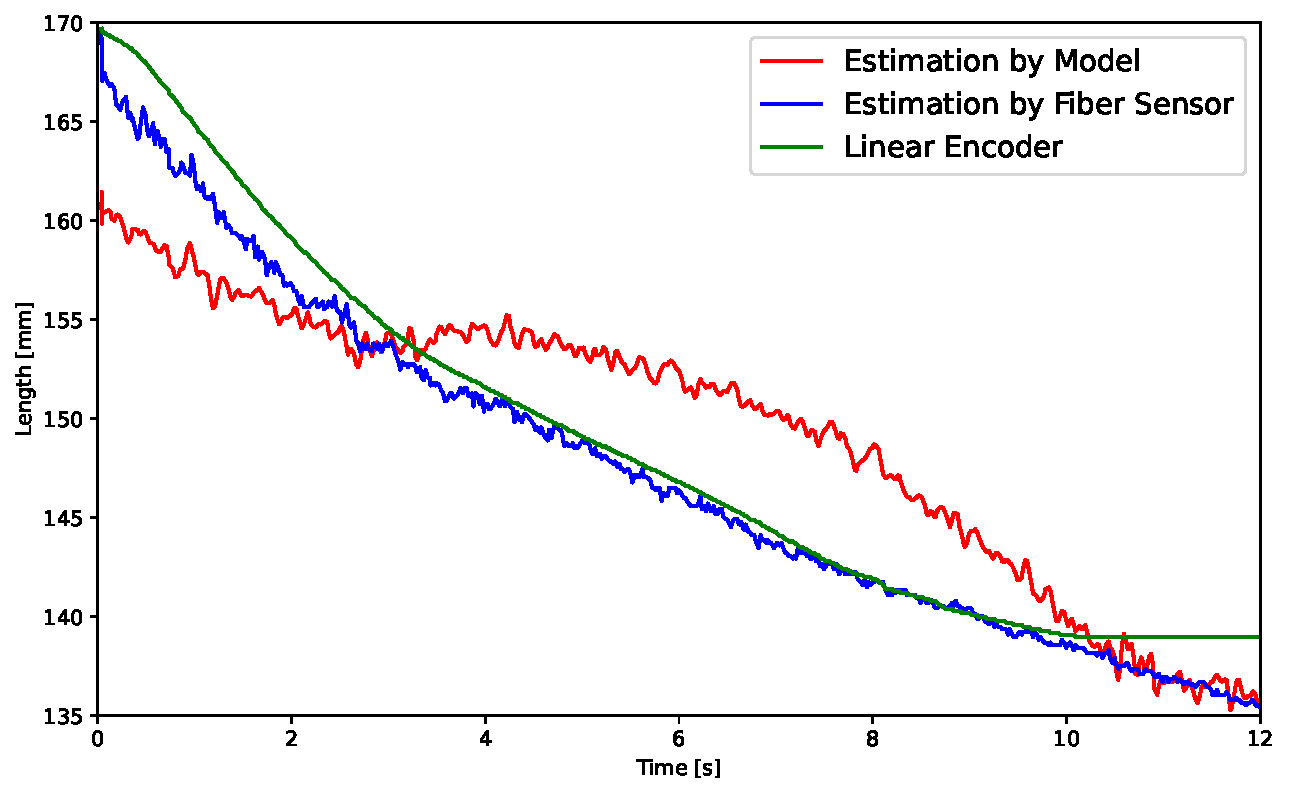
\includegraphics[width=\columnwidth]{fig/reaching_error.pdf}
            \caption{Length Estimation Error in Reaching Task}
            \label{fig:reaching_error}
            \vspace{1em}
            \addtocounter{figure}{1}
            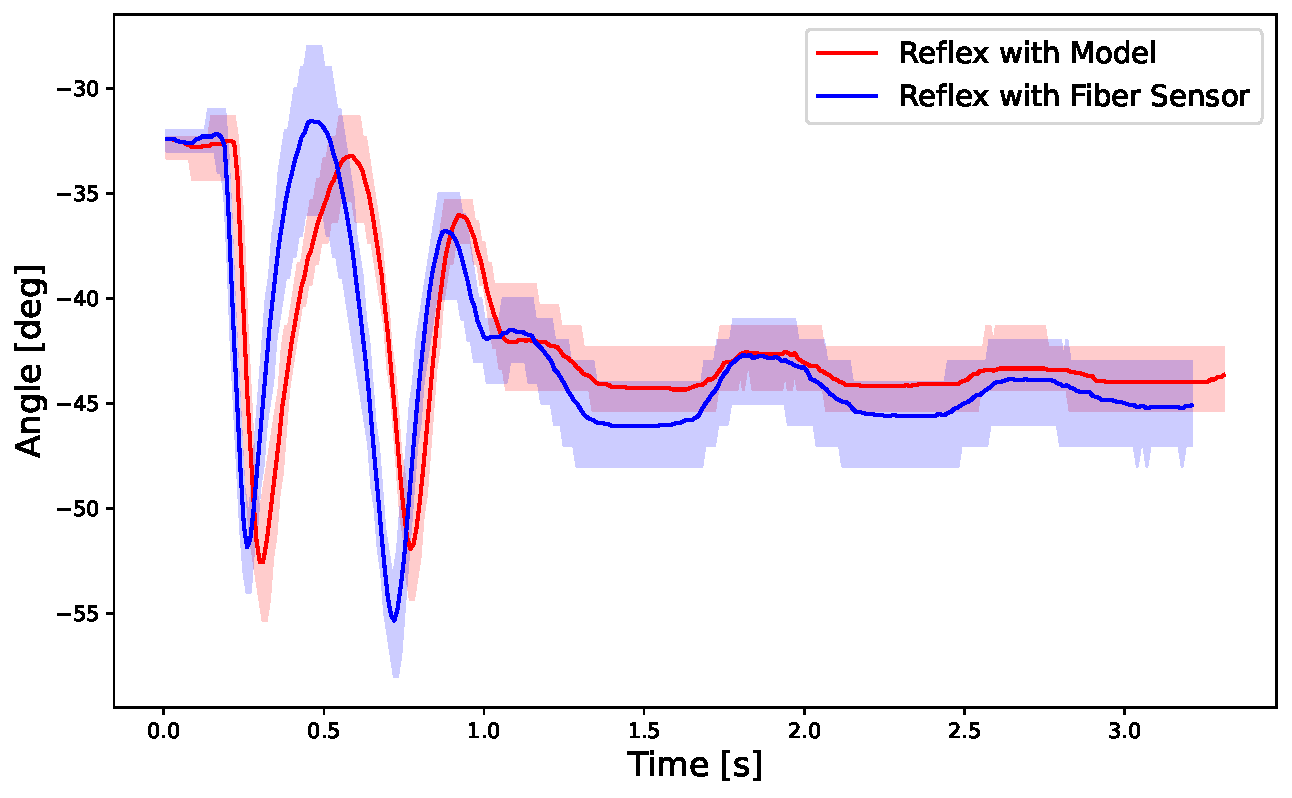
\includegraphics[width=\columnwidth]{fig/time_vs_angle_model_sensor.pdf}
            \caption{Reflex Angle Similarity between Model and Fiber Sensor}
            \label{fig:reflex_angle}
            \setcounter{figure}{7}  
            \renewcommand{\thefigure}{\arabic{figure}}  
        \end{minipage}
        \hfill
        \begin{minipage}[H]{0.48\textwidth} 
            \centering
            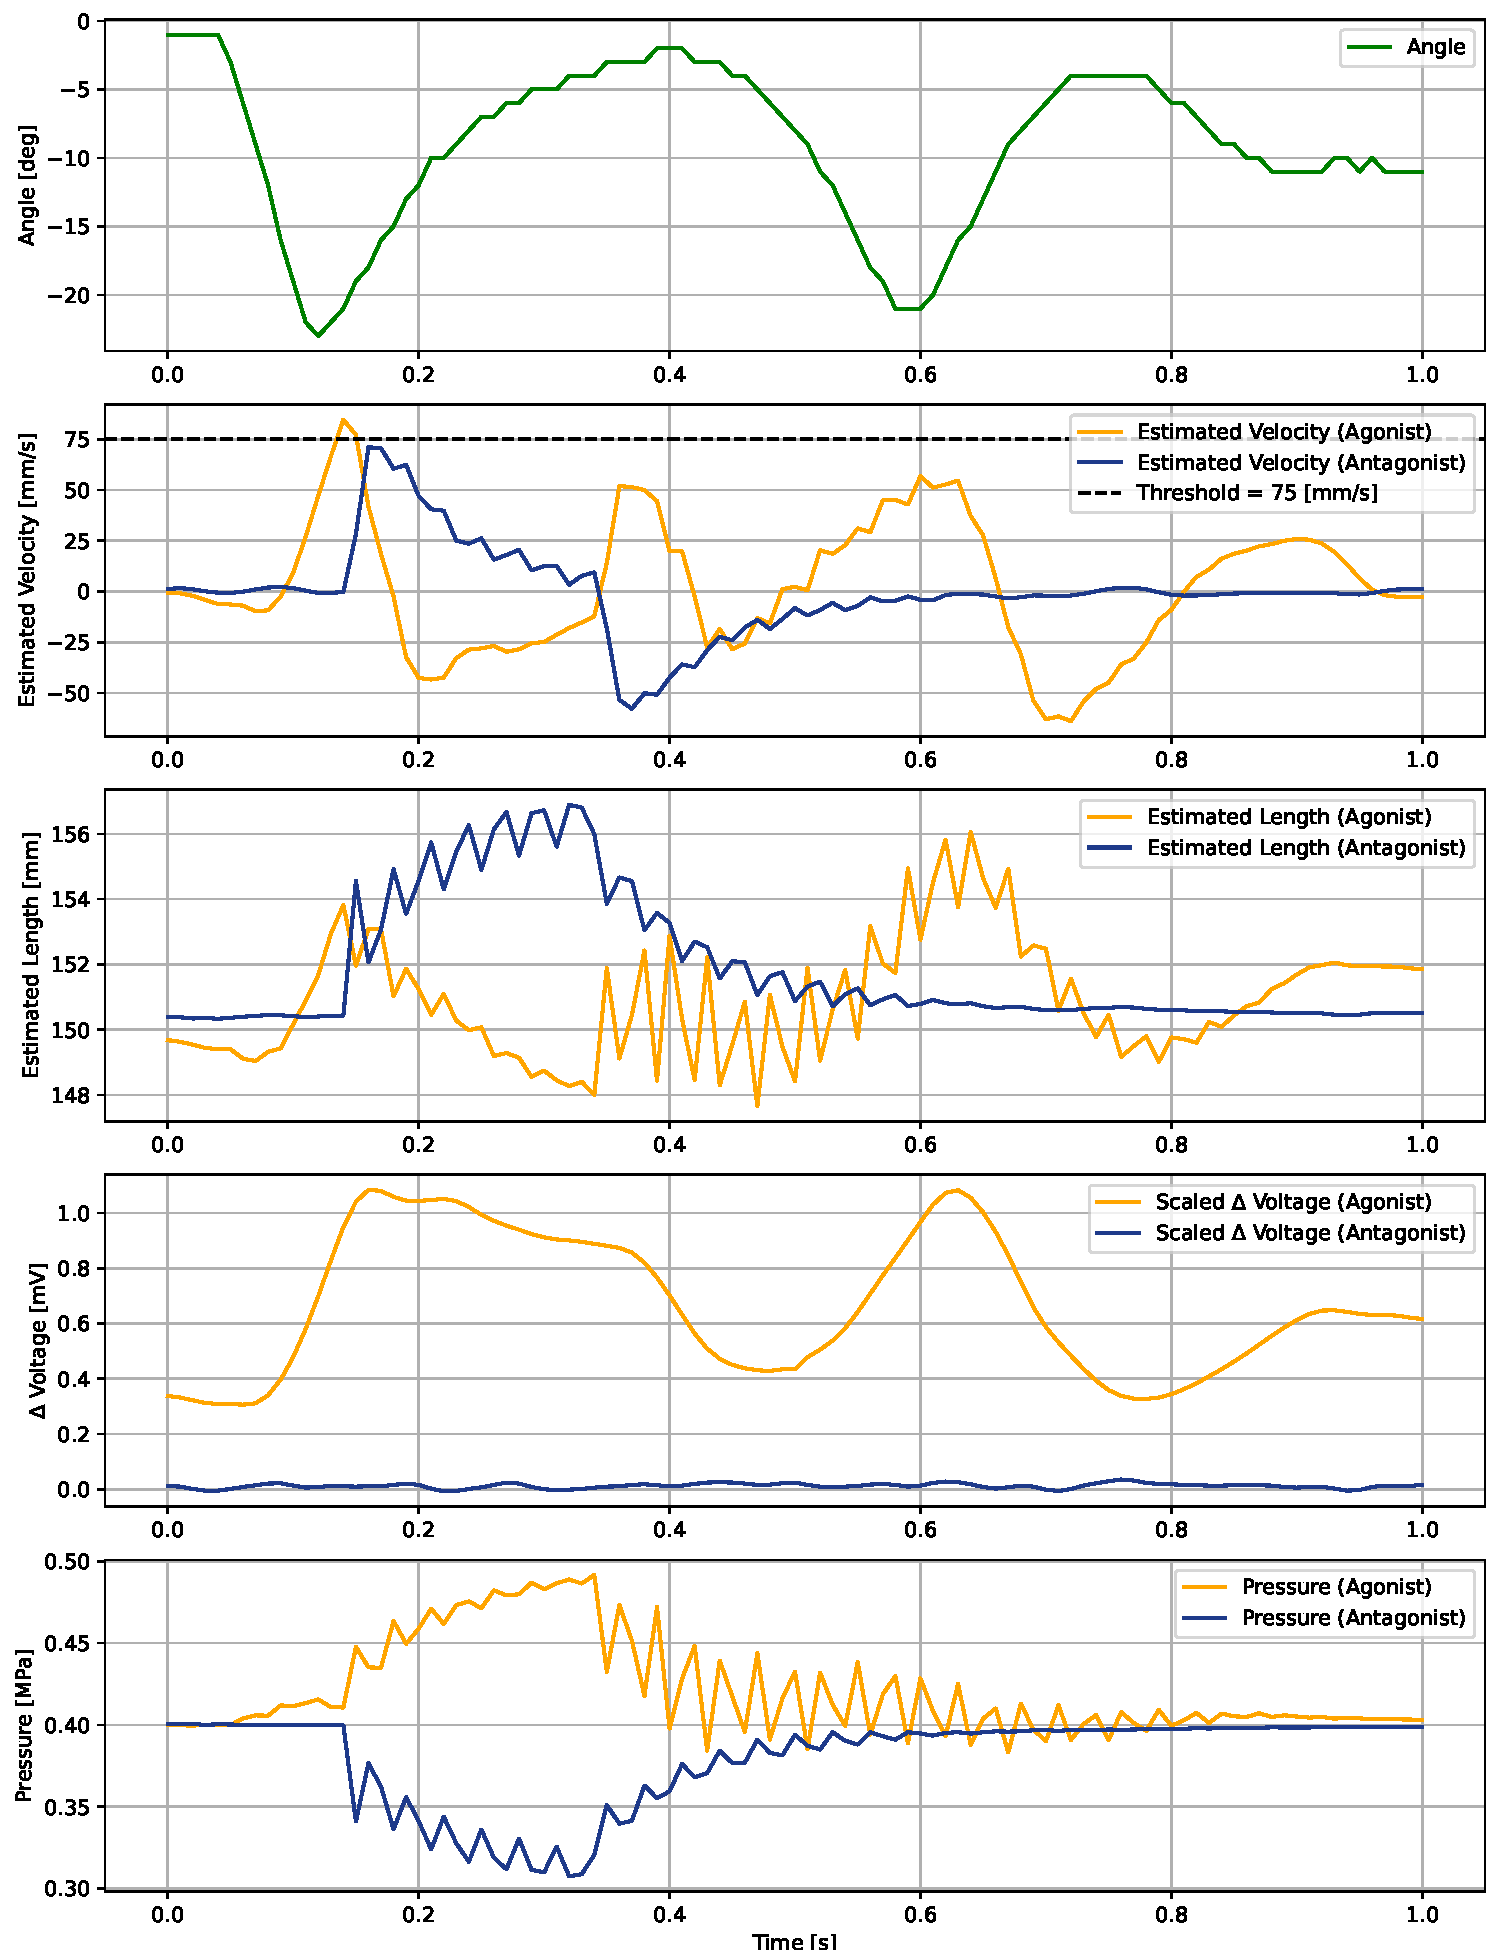
\includegraphics[width=\columnwidth]{fig/20240819_r20_reflex_all_plt.pdf}
            \caption{Dynamic Behavior of Reflex with Model}
            \label{fig:reflex_all}
            \setcounter{figure}{7}  
            \renewcommand{\thefigure}{\arabic{figure}} 
        \end{minipage}
    \end{minipage}
\end{figure*}

\subsection{Stretch Reflex}
Fig. \ref{fig:reflex_all} illustrates the dynamic behavior of the reflex with the model. With 0 degrees defined as the horizontal position of the arm and the positive rotational direction as clockwise in Fig. \ref{fig:reflex_equipment}, the starting angle was -36 degrees due to the attached basket's weight of 83.1 g. When the falling mass made an impact, the angle dropped dramatically, creating sudden soar in the voltage signal from the strain gauge and thus in estimated velocity. It went beyond the threshold and triggered the stretch reflex, leading to an increase in pressure in the agonist muscle and a decrease in the antagonist. The arm was then lifted back to the initial position, and after some oscillation, it settled down to a certain angle, holding the mass left in the basket.

Fig.\ref{fig:reflex_angle} displays the average and range of angles in 20 trials of the reflexes with the model and the fiber sensor. Since the thresholds and gains were determined experimentally, it is impossible to purely compare the behavior of the arm between the two reflexes, but it can be said that the reflex with the fiber sensor was well replicated with the model.



